\documentclass[11pt, fleqn]{article}

\usepackage[usenames,dvipsnames,svgnames,table]{xcolor}
\usepackage{amsmath}
\usepackage{amsfonts}
\usepackage[margin=1in]{geometry} % To set the margin widths
\usepackage{graphicx}
\usepackage{listings}
\usepackage{multirow}
\usepackage{tabularx}
\usepackage{varioref}
\usepackage[noabbrev,capitalize]{cleveref}
\usepackage[group-separator={,}]{siunitx}
\usepackage{subcaption}
\usepackage{titlesec}
\usepackage{lscape}
\usepackage{bm}
\usepackage{chngpage}
\usepackage[titletoc,toc,title]{appendix}

\renewcommand\thesection{\arabic{section}}
\renewcommand\thesubsection{\thesection\alph{subsection}}

\lstset{
  frame=single,
  basicstyle=\ttfamily,% print whole listing small
  language=R,
  aboveskip=3mm,
  belowskip=3mm,
  showstringspaces=false,
  columns=flexible,
  numbers=none,
  commentstyle=\color{ForestGreen},
  stringstyle=\color{Maroon},
  breaklines=true,
  breakatwhitespace=true,
  tabsize=2,
  literate={<-}{{$\gets$}}1 {~}{{$\sim$}}1
}

\sisetup{output-exponent-marker=\textsc{e}}

\setlength{\parskip}{12pt} % Sets a blank line in between paragraphs
\setlength\parindent{0pt} % Sets the indent for each paragraph to zero

\begin{document}

\title{Digital and Algorithmic Marketing (37304-01)\\Homework 2}
\author{Will Clark\\
University of Chicago Booth School of Business}
\date{\today}
\maketitle

\section{Comparing Recommendation Algorithm Performance} % Question 1

We used the \textsf{R} package \textsf{recommenderlab} to evaluate a user-based and an item-based recommendation model for the MovieLense data set. The data contain ratings from 943 users on 1664 movies where evaluations are made on a 1-5 scale.

To evaluate each algorithm, we repeated the following procedure five times:
\begin{itemize}
\item Randomly select 80 percent of the users to train the recommender on. The remaining 20 percent will be our hold-out sample.
\item For each of the users in the hold-out sample, randomly pick five movies that the user has seen and liked. For our purposes, a user ``likes'' a movie if s/he gives it at least a 4 out of 5.
\item Based on those 5 movies, let the recommender give a list of top $N$ movies the user might also like to see. We let $N=(1,3,5,10,15,20,50,100,150)$.
\item Compute accuracy statistics on the recommended movies.
\end{itemize}
This procedure gives us the average accuracy of each recommender algorithm across the five cuts of data. \cref{fig:accuracy} shows the accuracy of each recommender algorithm. The left panel shows the true positive rate against the false positive rate, and the right panel shows the precision against the recall (which is just another name for the true positive rate). A well performing algorithm will have a high true positive rate and a low false positive rate. As the right panel makes clear, an algorithm must trade off between high precision and high recall (it cannot have both).

\begin{figure}[!htb]
  \centering
  \caption{Recommendation Algorithm Accuracy}
  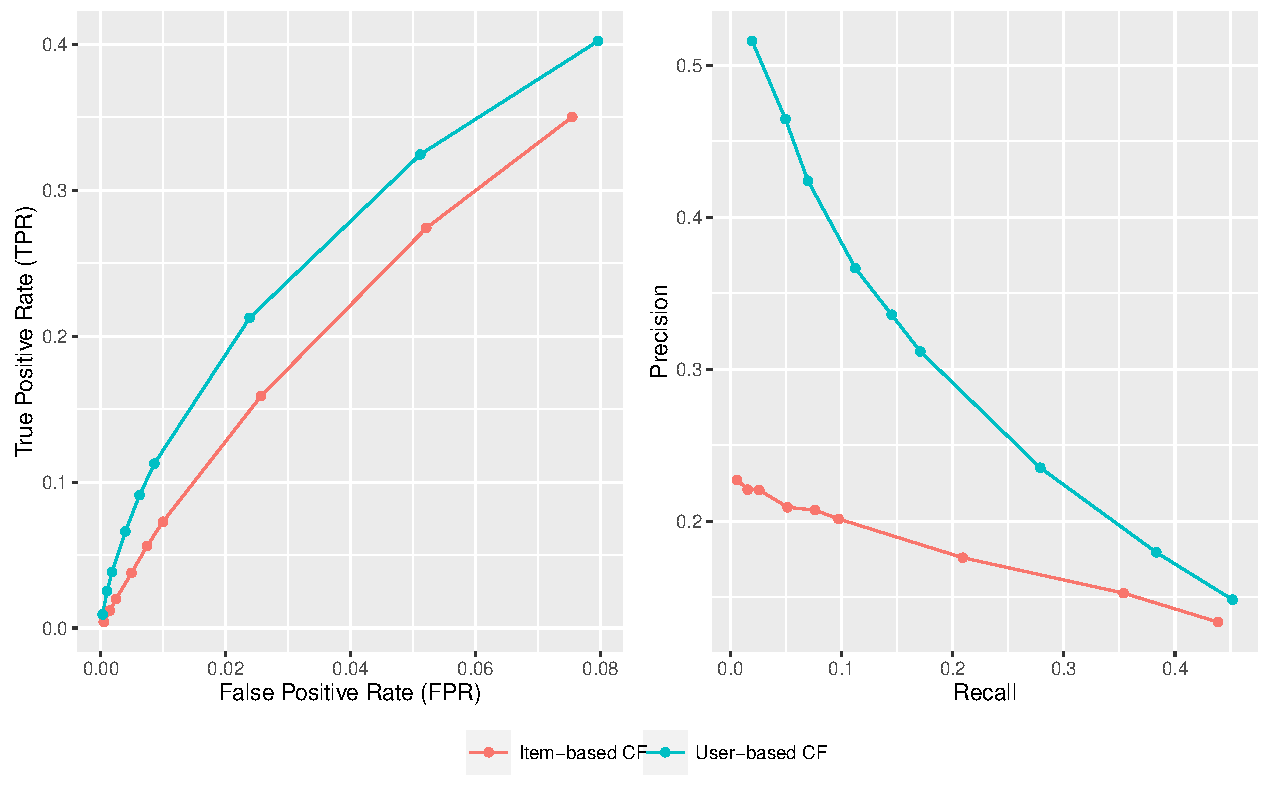
\includegraphics[scale=.65]{accuracy.pdf}
  \label{fig:accuracy}
\end{figure}

We can see from \cref{fig:accuracy} that the user-based recommendation algorithm performs better along all the relevant measures. It correctly identifies more movies that a user likes (true positive), minimizes the number of recommendations that a user \textit{doesn't} like (false positives), and has higher precision for a given level of recall than the item-based recommender.

The data are structured in such a way that the user-based recommendation algorithm should give us better predictions than the item-based algorithm. Consider that:
\begin{itemize}
\item the average user rates 105 movies and the median user rates 60 movies; and
\item the average movie is seen by 60 users and the median movie is seen by 27 users.
\end{itemize}
That is, if our recommendation algorithm is built on looking for similarity across either users or items, each user contains relatively more information than each item. We might expect, then, that the user-based algorithm gives us better results than the item-based algorithm.

In addition to performing better out of sample, the user-based recommendation algorithm can be fit much more quickly than the item-based algorithm. Across all five draws, the average time to fit for the user-based algorithm was 0.009 seconds, while the average time to fit for the item-based algorithm was 51.3 seconds.

\section{Overlap Between Recommendation Algorithms} % Question 2

We follow the procedure outlined in Section 1 above (split the data 80/20 into a training/test set, repeat five times) to test the overlap between the two recommendation algorithms. For all users in the test set across each draw, the average number of movies recommended by both algorithms 26.12 (out of 100 that were recommended).

We should expect to see some overlap in the data, though it is not obvious how much (that it was not higher than 26 surprised me a little bit). It would be strange if there were no overlap, as the algorithms are fundamentally trying to do the same thing: make a list of movies that a given user would like to see. 

Some of the overlap is caused by both algorithms recommending the same popular movies. To test this theory, we compared the average overlap of the 100 movies recommended by the two algorithms with the list of 100 most popular movies. On average, 8 of the 100 most popular movies are recommended by both algorithms. The user-based algorithm tends to recommend more of the popular movies (29 on average) than the item-based algorithm (14 on average).

\section{Ensemble Recommendation System} % Question 3

We could use this additional data to build a two-stage recommendation system. In the first stage, we could use the additional movie characteristics to build a logistic regression model to predict the likelihood that someone will enjoy a movie. We could choose from a few different techniques:
\begin{itemize}
\item a standard generalized linear regression, if the number of additional variables is sufficiently small;
\item a LASSO regression, which would algorithmically select which variables to include in the model;
\item a ridge regression, which would reduce the estimated effects of each variable in order to improve predictive accuracy; or
\item an elastic net regression, which also handles variable selection but would include more variables than the LASSO model.
\end{itemize}
Our preference would be for an elastic net regression, but we could imagine using cross-validation to see which model produces the best out-of-sample predictions. Note that this would be a kind of item-based similarity algorithm (although it is produced differently from the item-based collaborative filter used by \textsf{recommenderlab}).

In the second stage, we could use the user-based collaborative filtering algorithm discussed above. Rather than choosing a top-$N$ list, we could predict the average score that a user would give any movie. We could normalize these scores onto the unit interval so they would be scaled in the same way as the predictions made in the first stage.

Finally, we would weight the average of these two recommendation system. We would need to search over the range of possible weights for each stage, and we would select the weighting scheme that yields the most accurate set of predictions.


\end{document}


% \input{.tex}

% \begin{figure}[!htb]
%   \centering
%   \begin{subfigure}[b]{0.49\textwidth}
%     \caption{}
%     \includegraphics[width=\textwidth]{.pdf}
%     \label{fig:}
%   \end{subfigure}
%   \hfill
%   \begin{subfigure}[b]{0.49\textwidth}
%     \caption{}
%     \includegraphics[width=\textwidth]{.pdf}
%     \label{fig:}
%   \end{subfigure}
%   \caption{}
% \end{figure}

% \begin{figure}[!htb]
%   \centering
%   \caption{}
%   \includegraphics[scale=.5]{.pdf}
%   \label{fig:}
% \end{figure}
